\documentclass[border=10pt,tikz]{standalone}
\usepackage{tikz}
\usepackage{xcolor}
\usepackage[T1]{fontenc}
\usepackage{lmodern}
\usetikzlibrary{positioning,arrows.meta,decorations.pathreplacing,calc,fadings,shadows,backgrounds}

\definecolor{ink}{HTML}{0E1116}
\definecolor{inksoft}{HTML}{3A3F47}
\definecolor{inkmute}{HTML}{6A7079}
\definecolor{textc}{HTML}{2563EB}
\definecolor{audioc}{HTML}{EA580C}
\definecolor{accentc}{HTML}{7C3AED}
\definecolor{audiogreen}{HTML}{059669}
\definecolor{linec}{HTML}{CFC9B8}
\definecolor{soft}{HTML}{F3F1EA}

\begin{document}
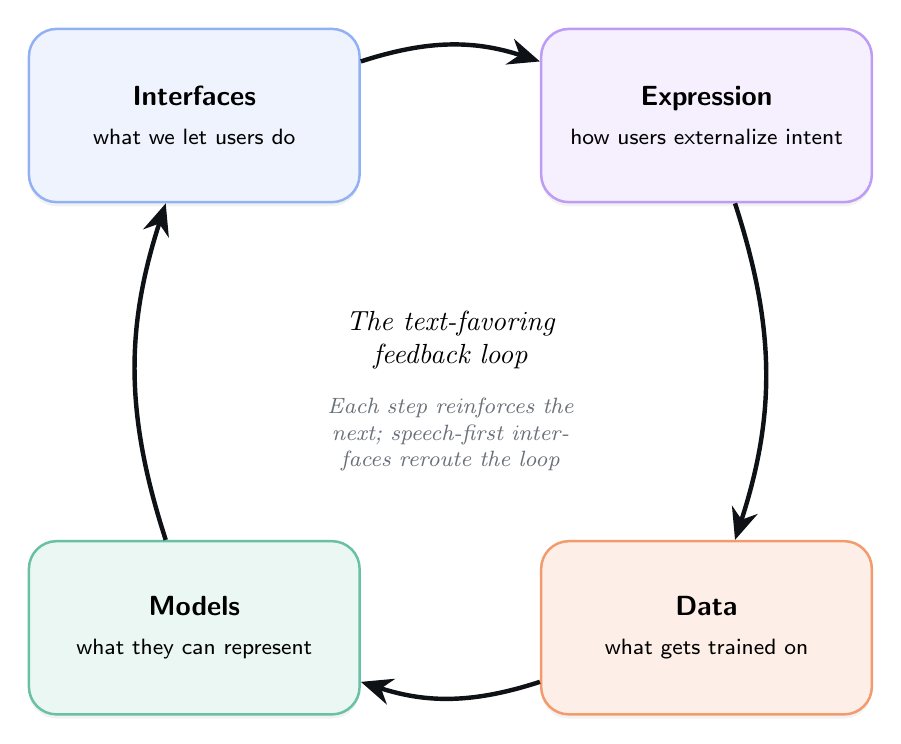
\begin{tikzpicture}[
  font=\sffamily,
  every node/.style={font=\sffamily},
  node/.style={
    rectangle, rounded corners=10pt,
    draw=ink, line width=0.9pt,
    fill=white, drop shadow={shadow xshift=0pt, shadow yshift=-1.5pt, opacity=0.10},
    minimum height=22mm, minimum width=42mm, align=center,
    inner sep=8pt
  },
  arr/.style={->, >={Stealth[length=4mm,width=3.4mm]}, line width=1.6pt, draw=ink},
  curvedarr/.style={->, >={Stealth[length=4mm,width=3.4mm]}, line width=1.6pt, draw=ink}
]

% Four nodes around a circle
\def\R{4.6}
\node[node, fill=textc!8, draw=textc!50] (interfaces)  at ({\R*cos(135)}, {\R*sin(135)})  {\textbf{Interfaces}\\[2pt]\footnotesize what we let users do};
\node[node, fill=accentc!8, draw=accentc!50] (expression)  at ({\R*cos(45)},  {\R*sin(45)})   {\textbf{Expression}\\[2pt]\footnotesize how users externalize intent};
\node[node, fill=audioc!10, draw=audioc!60]  (data)        at ({\R*cos(-45)}, {\R*sin(-45)})  {\textbf{Data}\\[2pt]\footnotesize what gets trained on};
\node[node, fill=audiogreen!8, draw=audiogreen!60] (models) at ({\R*cos(-135)},{\R*sin(-135)}) {\textbf{Models}\\[2pt]\footnotesize what they can represent};

% Curved arrows between them
\draw[curvedarr] (interfaces) to[bend left=18] (expression);
\draw[curvedarr] (expression) to[bend left=18] (data);
\draw[curvedarr] (data)        to[bend left=18] (models);
\draw[curvedarr] (models)      to[bend left=18] (interfaces);

% Center label
\node[align=center, font=\itshape] at (0,0.4) {The text-favoring\\feedback loop};
\node[align=center, font=\footnotesize\itshape, color=inkmute, text width=4cm] at (0,-0.8) {Each step reinforces the next; speech-first interfaces reroute the loop};

\end{tikzpicture}
\end{document}
